\documentclass{report}

\usepackage{amsmath, amssymb, amsfonts}
%\usepackage{pdfsync}
\usepackage{graphicx,subcaption,verbatim}
%\usepackage{fancyhdr}

\usepackage{tikz}
\usepackage[forpaper, %
useforms , 
%nosolutions, pointsonleft
nopoints,answerkey
]{eqexam}

\usetikzlibrary{calc,arrows}
%\usepackage[usenames]{color}
%\definecolor{myblue}{rgb}{.2, .2, .7}

\usepackage{pgfplots}
\pgfplotsset{compat=newest}

\newcommand\dsp{\displaystyle}

\newcommand{\norm}[1]{\left\Vert #1 \right\Vert}
\newcommand{\avec}[1]{\left\langle #1 \right\rangle}
\newcommand{\Reals}{\mathbb{R}}
\newcommand{\vect}[1]{\overrightarrow{#1}}
\newcommand{\abs}[1]{\left\vert{#1}\right\vert}

\rheadeqe{} % no name on pages other than first



\title[MT1]{Midterm Exam 1} %\author{O. Bastille}
\subject{MATH253X-F01} 
\examNameLabel{Name:}
%\date{\thisterm\space\the\year}
\date{Summer\space2016}

\chead{-- Page \arabic{page}\space of \eqExamLastPage\space--}

\begin{document}\maketitle

% Formal beginning of the exam.
\begin{exam}{Part1}
\begin{instructions}
You have 90 minutes. No calculators allowed. \emph{Show all your work} in order to receive full credit.
\end{instructions}

%-------------------------------Problem 1------------------------------
\begin{problem*}[\auto] Consider the points $A(2,1,0)$, $B(-1,3,1)$, $C(0,4,-1)$, and $D(1,-1,2)$ in space.

\begin{center}
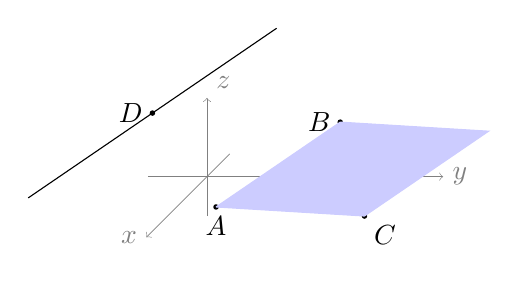
\begin{tikzpicture}[scale=0.5]
% in 3D, (0,0,1) is i; (1,0,0) is j and (0,1,0) is k
\draw[help lines,->] (-1.5,0,0) -- (6,0,0) node[right] {$y$};
\draw[help lines,->] (0,-1,0) -- (0,2,0) node[above right] {$z$};
\draw[help lines,->] (0,0,-1.5) -- (0,0,4) node[left] {$x$};
\coordinate (a) at (1,0,2);
\coordinate (b) at (3,1,-1);
\coordinate (c) at (4,-1,0);
\coordinate (d) at (-1,2,1);
\fill (a) circle (2pt) node[below] {$A$} % point (0,1,2)
      (b) circle (2pt) node[left] {$B$} % point (2,-1,3)
      (c) circle (2pt) node[below right] {$C$}% point (2,1,1)
      (d) circle (2pt) node[left] {$D$} % point (-1,1,1)
      ;
      
\filldraw[blue!20] (a) -- (b) -- ($(c)+(b)-(a)$) -- (c) -- (a); % -- (d) -- ($(d)+(c)-(a)$) -- ($(d)+(c)+(b)-2*(a)$) -- ($(c)+(b)-(a)$)
%(c) -- ($(d)+(c)-(a)$);
\draw ($(d)-(b)+(a)$) -- (d) -- ($(d)+(b)-(a)$);
%\draw[dotted] (0,2,0) -- (p) -- (1,0,0)
%			  (q) -- (-1,0,2) -- (-1,0,0)
%			  (-1,0,2) -- (0,0,2)
%			  (r) -- (1,0,2) -- (0,0,2)
%			  (1,0,2) -- (1,0,0) -- (1,0,-1) -- (s)
%			  (1,0,-1) -- (0,0,-1);      
\end{tikzpicture}

\end{center}

\begin{parts}
\item\PTs{6} Find the symmetric equations of the line going through $D$ and parallel to the line going through $A$ and $B$.
\begin{solution}[1.5in] The direction for the line will be (any scalar multiple of):
$$\vect{AB}=\avec{-1-2,3-1,1-0}=\avec{-3,2,1} $$
And symmetric equations for the line through $D$ parallel to $\vect{AB}$ are:
$$\boxed{\dfrac{x-1}{-3}=\dfrac{y+1}{2}=z-2}$$
\end{solution}
\item\PTs{8} Find the equation of the plane containing the parallelogram shaded above.
\begin{solution}[2.5in] A normal vector to the plane is:
\begin{align*}
\vect{AB}\times\vect{AC}&=\avec{-3,2,1}\times\avec{0-2,4-1,-1-0}=\avec{-3,2,1}\times\avec{-2,3,-1}\\
&=\begin{vmatrix}
\mathbf{i} & \mathbf{j} & \mathbf{k} \\
-3 & 2 & 1 \\
-2 & 3 & -1
\end{vmatrix}=\avec{2(-1)-3(1),-(-3(-1)+2(1)),-3(3)+2(2)}=\avec{-5,-5,-5}. 
\end{align*}
A more judicious choice is $\avec{1,1,1}$ and then the equation to the plane is:
$$\boxed{(x-2)+(y-1)+z=0}\quad\text{ or equivalently }\quad \boxed{x+y+z=3}. $$
\end{solution}
\item\PTs{6} Use vectors to find the length of the diagonal starting at $A$ in the parallelogram. 
\begin{solution}[1.5in]
A vector representing the diagonal is $\vect{AB}+\vect{AC}$ so the length of the diagonal is:
\begin{align*}
\norm{\vect{AB}+\vect{AC}}&=\norm{\avec{-3,2,1}+\avec{-2,3,-1}}=\norm{\avec{-3-2,2+3,1-1}}=\norm{\avec{-5,5,0}}\\
&=\sqrt{25+25+0}=\sqrt{50}=\boxed{5\sqrt{2}}.
\end{align*}
\end{solution}

\end{parts}
\end{problem*}

%---------------------------Problem 2------------------------------
%\newpage
\begin{problem*}[\auto] Consider the following planes in space:
$$\begin{matrix}
\text{Plane 1} & x-2y-\phantom{2}z+1=0 \\
\text{Plane 2} & x-3y+2z+6=0
\end{matrix}$$
\begin{parts}
\item\PTs{5} Are the two planes orthogonal?
\begin{solution}[2in] We need to compute the dot product of the normal vectors:
$$\avec{1,-2,-1}\cdot\avec{1,-3,2}=1(1)-2(-3)-1(2)=5\ne 0 $$
so \fbox{the planes are not orthogonal}.
\end{solution}
\item\PTs{5} Find the point of intersection of Plane 1 and the line parametrized by $$\vec{r}(t)=\avec{-2+t,1-t,3+2t}.$$
\begin{solution}[2in] Substitute $x$, $y$, and $z$ with the parametrization of the line in Plane 1 and solve for $t$:
$$(-2+t)-2(1-t)-(3+2t)+1=0 \quad \Longleftrightarrow\quad -2+t-2+2t-3-2t+1=0 \quad \Longleftrightarrow\quad t=6.$$
Thus, we have
$$\vect{r}(6)=\avec{-2+6,1-6,3+2(6)}=\avec{4,-5,15}\quad \Longrightarrow\quad \boxed{P(4,-5,15)}. $$
\end{solution}
\item\PTs{5} Now find the distance from the point found above to Plane 2.
\begin{solution}[2in]
$$d=\dfrac{\abs{4-3(-5)+2(15)+6}}{\norm{\avec{1,-3,2}}}=\frac{\abs{4+15+30+6}}{\sqrt{1+9+4}}=\frac{55}{\sqrt{14}}=\boxed{\frac{55\sqrt{14}}{14}} $$
\end{solution}
\end{parts}
\end{problem*}

%-------------------------------Problem 3-------------------------
%\newpage

\begin{problem*}[\auto]Let $\mathbf{r}(t)=\avec{(t-1)^2,t^3-3t^2+3t,2t^3-3t^2}$ be describing the motion of a particle along a space curve over time. The position is in meters and time in seconds.
\begin{parts}
%\item\PTs{3} Show that the particle stays on the plane given by the equation:
%$$3x-2y+z-3=0. $$
%\begin{solution}[2.25in]
%\end{solution}
\item\PTs{3} Find all the open intervals on which the curve is smooth.
\begin{solution}[2.5in]
The domain of $\mathbf{r}(t)$ is the whole real line, and $$\mathbf{r^\prime}(t)=\avec{2(t-1),3t^2-6t+3,6t^2-6t}=\avec{2(t-1),3(t-1)^2,6t(t-1)}$$ is defined, and continuous also on the whole real line. But 
$$\mathbf{r^\prime}(t)=\vect{0} \quad \text{ for }\quad t=1$$
So by definition,
$$\boxed{\text{the curve described by }\vec{r}(t) \text{ is smooth on }(-\infty,1)\cup(1,\infty).}$$
\end{solution}
\item\PTs{4} Find the speed of the particle at $t=2$ s.
\begin{solution}[2.5in] 
$$\norm{\mathbf{r'}(2)}=\norm{\avec{2(1),3(1)^2,6(2)(1)}}=\norm{\avec{2,3,12}}=\sqrt{4+9+144}=\boxed{\sqrt{157}\text{ m/s}.} $$
\end{solution}
\item\PTs{3} Given $\mathbf{s}(2)=\avec{2,3,-1}$ and $\mathbf{s'}(2)=\avec{1,-1,2}$, find:
\vskip0.2in
\begin{enumerate}
\item $\left.\dfrac{d\phantom{t}}{dt}\left(\mathbf{r} \cdot \mathbf{s} \right)\right|_{t=2}= $\fillin[b]{1in}{ $\boxed{8}$}
\begin{solution}[1in]
\begin{align*}
\left.\dfrac{d\phantom{t}}{dt}\left(\mathbf{r} \cdot \mathbf{s} \right)\right|_{t=2}&= (\mathbf{r'}\cdot\mathbf{s}+\mathbf{r}\cdot\mathbf{s'})\Big|_{t=2}=\avec{2,3,12}\cdot\avec{2,3,-1}+\avec{1^2,8-12+6,16-12}\cdot\avec{1,-1,2}\\
&=2(2)+3(3)+12(-1)+\avec{1,2,4}\cdot\avec{1,-1,2}=4+9-12+1(1)+2(-1)+4(2)\\
&=1+1-2+8=8
\end{align*}
\end{solution}

\item $\left.\dfrac{d\phantom{t}}{dt}\left(\mathbf{r} \times \mathbf{s} \right)\right|_{t=2}= $ \fillin[b]{1in}{ $\boxed{\avec{-31,28,-3}}$}
\begin{solution}[0.5in]
\begin{align*}
\left.\dfrac{d\phantom{t}}{dt}\left(\mathbf{r} \times \mathbf{s} \right)\right|_{t=2}&= (\mathbf{r'}\times\mathbf{s}+\mathbf{r}\times\mathbf{s'})\Big|_{t=2}=\avec{2,3,12}\times\avec{2,3,-1}+\avec{1,2,4}\times\avec{1,-1,2}\\
&=\begin{vmatrix}
\mathbf{i} & \mathbf{j} & \mathbf{k} \\
2 & 3 & 12 \\
2 & 3 & -1
\end{vmatrix}+\begin{vmatrix}
\mathbf{i} & \mathbf{j} & \mathbf{k} \\
1 & 2 & 4 \\
1 & -1 & 2
\end{vmatrix} \\
&=\avec{3(-1)-3(12),-(2(-1)-2(12)),2(3)-2(3)}\\
&\qquad\qquad+\avec{2(2)+1(4),-(1(2)-1(4)),1(-1)-1(2)}\\
&=\avec{-39,26,0}+\avec{8,2,-3}=\avec{-31,28,-3}
\end{align*}
\end{solution}
\end{enumerate}
\end{parts}
\end{problem*}

%---------------------------Problem 4--------------------------
%\newpage
\begin{problem*}[\auto] Time to sketch some surfaces!

\begin{parts}

%\item\PTs{8} Convert the point $P$ with spherical coordinates $P\left(3, \frac{\pi}{3}, \frac{3\pi}{4}\right)$ to rectangular coordinates.

%\begin{solution}[3.5in]
%We have $r=3$, $\theta=\frac{\pi}{6}$, and $z=1$. So in rectangular coordinates,
%$$\begin{cases}
%x=r\cos\theta=\frac{3\sqrt{3}}{2} \\
%y=r\sin\theta=\frac{3}{2} \\
%z=z=1
%\end{cases}\quad, \text{ therefore }\quad \boxed{P\left(\frac{3\sqrt{3}}{2},\frac{3}{2},1\right)} \text{ in rectangular coordinates.} $$
%\end{solution}

\item\PTs{4} Describe and sketch the surface in space whose equation is $x^2-\dfrac{y^2}{4}+\dfrac{z^2}{9}=-1$.


\begin{solution}[2in] \fbox{hyperboloid of two sheets}
	\begin{center}
			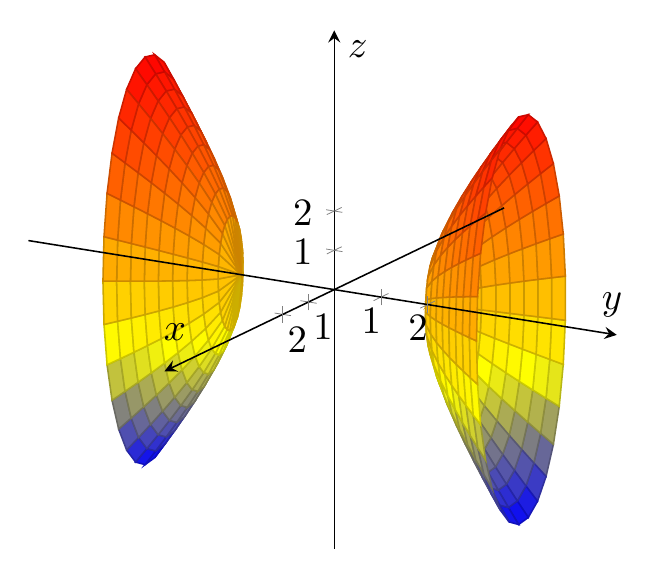
\begin{tikzpicture}[scale=1.4]
						\begin{axis}[
						width=10cm, view={120}{20},
						axis on top,
						axis lines=center,
						enlargelimits=.1,
						ymin=-5.5, ymax=5, xmin=-5.5, xmax=5.5, zmin=-5.5, zmax=5.5,
						xlabel=$x$, ylabel=$y$, zlabel=$z$, xtick={1,2},ytick={1,2},ztick={1,2}
						]
						\addplot3[surf,domain=0:360,y domain=-4:-2,samples=30,samples y=10,z buffer=sort] ({sqrt(y*y/4-1)*cos(x)},y,{3*sqrt(y*y/4-1)*sin(x)});
						\addplot3[surf,domain=0:360,y domain=2:4,samples=30,samples y=10,z buffer=sort] ({sqrt(y*y/4-1)*cos(x)},y,{3*sqrt(y*y/4-1)*sin(x)});
						\end{axis}
						\end{tikzpicture}
						\end{center}
\end{solution}

\item\PTs{4} Describe and sketch the surface in space whose equation is: $x^2+4y^2=z$.

\begin{solution}[2in] \fbox{elliptic paraboloid}
\begin{center}
			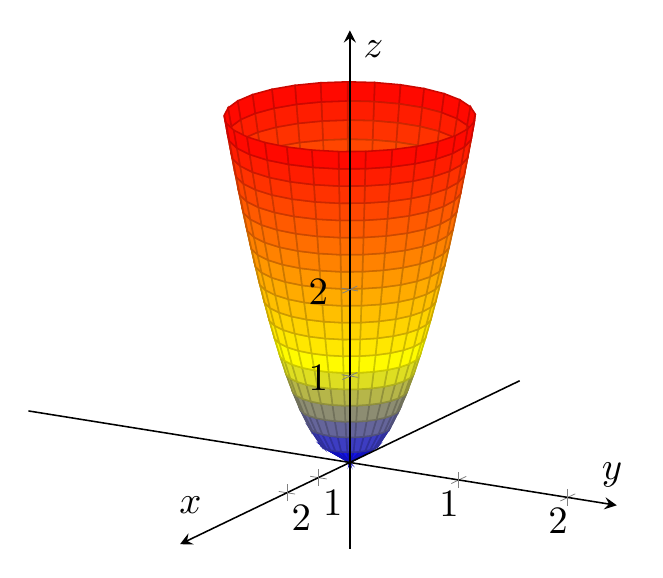
\begin{tikzpicture}[scale=1.4]
						\begin{axis}[
						width=10cm, view={120}{20},
						axis on top,
						axis lines=center,
						enlargelimits=.1,
						ymin=-2.5, ymax=2, xmin=-4.5, xmax=4.5, zmin=-0.5, zmax=4.5,
						xlabel=$x$, ylabel=$y$, zlabel=$z$, xtick={1,2},ytick={1,2},ztick={1,2}
						]
						\addplot3[surf,domain=0:360,y domain=0:4,samples=30,samples y=20,z buffer=sort] ({sqrt(y)*cos(x)},{0.5*sqrt(y)*sin(x)},y);
						\end{axis}
						\end{tikzpicture}
						\end{center}
\end{solution}
\end{parts}
\end{problem*}

\begin{problem}[7] You hit a golf ball in ``Calculus III conditions"\footnote{I.e. the acceleration is constant and only due to gravity. That is we ignore ball spin, air resistance, etc.} such that it takes off at an angle of $30^\circ$ with the horizontal. What should the initial golf ball speed be in order for you to hit a hole-in-one located 800 feet away at the same elevation?
\begin{solution}[2in] Let $v_0$ be the original speed. Then the initial velocity is $$\mathbf{v}(0)=\avec{v_0\cos30^{\circ},v_0\sin30^{\circ}}=\avec{\dfrac{v_0\sqrt{3}}{2},\dfrac{v_0}{2}}$$ and since the initial position is $\mathbf{r}(0)=\avec{0,0}$, we have:
\begin{align*}
\mathbf{a}(t)&=\avec{0,-32} \quad\Longrightarrow\quad \mathbf{v}(t)-\mathbf{v}(0)=\int_0^t\avec{0,-32}\;du=\avec{0,-32u}\Big|_{u=0}^{u=t}=\avec{0,-32t}\\
\Longleftrightarrow\quad \mathbf{v}(t) &=\avec{\dfrac{v_0\sqrt{3}}{2},\dfrac{v_0}{2}}+\avec{0,-32t}=\avec{\dfrac{v_0\sqrt{3}}{2},\dfrac{v_0}{2}-32t}\\
\Longrightarrow\quad \mathbf{r}(t)-\mathbf{r}(0) &= \int_0^t \avec{\dfrac{v_0\sqrt{3}}{2},\dfrac{v_0}{2}-32u}\;du=\left. \avec{\dfrac{v_0u\sqrt{3}}{2},\dfrac{v_0u}{2}-16u^2}\right|_{u=0}^{u=t}\\
\Longrightarrow\quad \mathbf{r}(t) &=  \avec{\dfrac{v_0t\sqrt{3}}{2},\dfrac{v_0t}{2}-16t^2}
\end{align*}
Now we solve for $t$ and $v_0$ in $\mathbf{r}(t)=\avec{800,0}$. From the $y$-component,
$$\frac{v_0t}{2}=16t^2 \quad\Longleftrightarrow\quad t=0\quad \text{ or }\quad t=\frac{v_0}{32} $$
and since $t=0$ just gives $\mathbf{r}(0)=\avec{0,0}$, here we need the second value of $t$ and thus we solve from the $x$-component:
$$800=\frac{v_0^2\sqrt{3}}{64} \quad\Longleftrightarrow\quad v_0=\sqrt{\frac{800(64)}{\sqrt{3}}}=\boxed{\frac{160\sqrt{2}}{\sqrt[4]{3}}\text{ ft/s}}$$
\end{solution} 
	\end{problem}



%\newpage
%--------------------------Problem 8-----------------------------------------------
\begin{problem*}[\auto] An object moves along a trajectory so that its position $\vect{r}(t)$ as a function of time is given by:
$$\vect{r}(t)=\avec{2\sin(\sqrt{6}t),2\cos(\sqrt{6}t),t}. $$
\begin{parts}
\item\PTs{5} The particle's trajectory sits on the intersection of the cylinder $y=2\cos(\sqrt{6}z)$ (drawn below) and which other surface? Sketch that surface.
(\emph{Hint:} Even though there is more than one possible answer, one is definitely easier to sketch.)
\begin{solution}[3in]

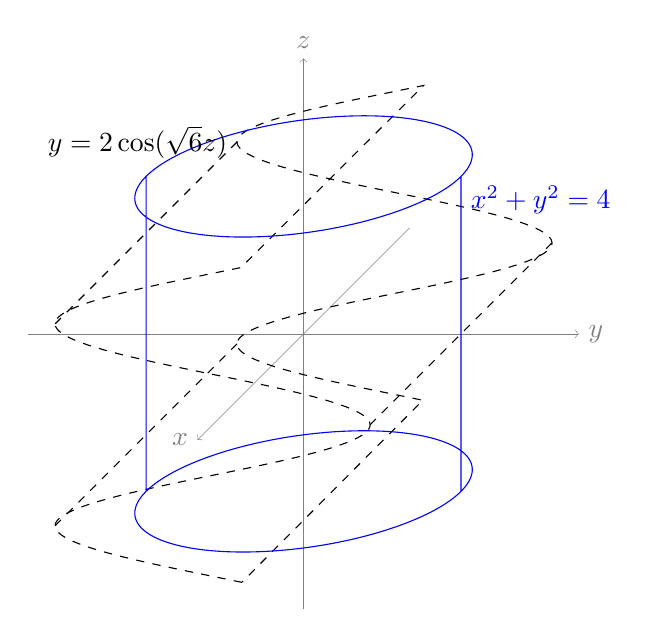
\begin{tikzpicture}[scale=1]
% in 3D, (0,0,1) is i; (1,0,0) is j and (0,1,0) is k
\draw[help lines,->] (-3.5,0,0) -- (3.5,0,0) node[right] {$y$};
\draw[help lines,->] (0,-3.5,0) -- (0,3.5,0) node[above] {$z$};
\draw[help lines,->] (0,0,-3.5) -- (0,0,3.5) node[left] {$x$};
\draw[dashed,domain=-2:2,samples=1000,variable=\t] plot ({2*(cos(sqrt(6)*\t r))},{\t},{3}) -- ($cos(sqrt(24) r)*(2,0,0)+(0,2,-3)$) -- plot ({2*(cos(sqrt(6)*\t r))},{-\t},{-3})
-- ($cos(sqrt(24) r)*(2,0,0)+(0,-2,3)$);
%\draw ($cos(sqrt(24) r)*(2,0,0)+(0,2,3)$)  -- ($cos(sqrt(24) r)*(2,0,0)+(0,2,-3)$);
%\draw ($cos(sqrt(24) r)*(2,0,0)+(0,-2,3)$)  -- ($cos(sqrt(24) r)*(2,0,0)+(0,-2,-3)$);
\draw[blue,domain=0:360,samples=500,variable=\t] (2,-2,0) -- plot ({2*cos(\t)},-2,{2*sin(\t)}) --  (2,2,0) node[below right] {$x^2+y^2=4$} -- plot ({2*cos(\t)},2,{2*sin(\t)}) 
(-2,2,0) -- (-2,-2,0);
\draw[dashed] ($pi/sqrt(6)*(0,1,0)+(-2,0,3)$) -- ($pi/sqrt(6)*(0,1,0)+(-2,0,-3)$) node[left] {$y=2\cos(\sqrt{6}z)$};
\draw[dashed] ($pi/sqrt(6)*(0,-1,0)+(-2,0,3)$) -- ($pi/sqrt(6)*(0,-1,0)+(-2,0,-3)$) ;
\draw[dashed] (2,0,3) -- (2,0,-3) ;
\end{tikzpicture}\hspace{0.2cm}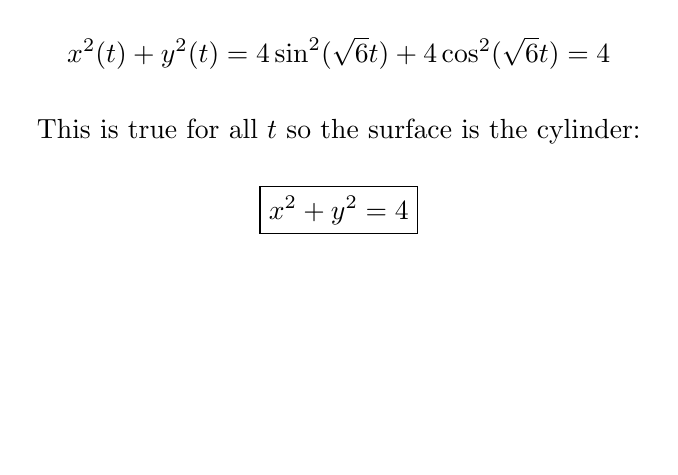
\begin{tikzpicture}[baseline=-2cm]
\draw  (0,3) node {$x^2(t)+y^2(t)=4\sin^2(\sqrt{6}t)+4\cos^2(\sqrt{6}t)=4$};
\draw (0,2) node {This is true for all $t$ so the surface is the cylinder:};
\draw (0,1) node {$\boxed{x^2+y^2=4}$};
\end{tikzpicture}
\end{solution}
\begin{workarea}{3in}
%\begin{center}
\begin{tikzpicture}[scale=1]
% in 3D, (0,0,1) is i; (1,0,0) is j and (0,1,0) is k
\draw[help lines,->] (-3.5,0,0) -- (3.5,0,0) node[right] {$y$};
\draw[help lines,->] (0,-3.5,0) -- (0,3.5,0) node[above] {$z$};
\draw[help lines,->] (0,0,-3.5) -- (0,0,3.5) node[left] {$x$};
\draw[dashed,domain=-2:2,samples=1000,variable=\t] plot ({2*(cos(sqrt(6)*\t r))},{\t},{3}) -- ($cos(sqrt(24) r)*(2,0,0)+(0,2,-3)$) -- plot ({2*(cos(sqrt(6)*\t r))},{-\t},{-3})
-- ($cos(sqrt(24) r)*(2,0,0)+(0,-2,3)$);
%\draw ($cos(sqrt(24) r)*(2,0,0)+(0,2,3)$)  -- ($cos(sqrt(24) r)*(2,0,0)+(0,2,-3)$);
%\draw ($cos(sqrt(24) r)*(2,0,0)+(0,-2,3)$)  -- ($cos(sqrt(24) r)*(2,0,0)+(0,-2,-3)$);
\draw[dashed] ($pi/sqrt(6)*(0,1,0)+(-2,0,3)$) -- ($pi/sqrt(6)*(0,1,0)+(-2,0,-3)$) node[left] {$y=2\cos(\sqrt{6}z)$};
\draw[dashed] ($pi/sqrt(6)*(0,-1,0)+(-2,0,3)$) -- ($pi/sqrt(6)*(0,-1,0)+(-2,0,-3)$) ;
\draw[dashed] (2,0,3) -- (2,0,-3) ;
\end{tikzpicture}
%\end{center}
\end{workarea}
\item\PTs{5}Find the unit tangent vector of the trajectory.
\begin{solution}[2in] 
\begin{align*}
\vect{r'}(t)&=\avec{2\sqrt{6}\cos(\sqrt{6}t),-2\sqrt{6}\sin(\sqrt{6}t),1} \\
\Longrightarrow\quad \vect{T}(t)&=\frac{\vect{r'}(t)}{\norm{\vect{r'}(t)}}=\frac{\avec{2\sqrt{6}\cos(\sqrt{6}t),-2\sqrt{6}\sin(\sqrt{6}t),1}}{\sqrt{24\cos^2(\sqrt{6}t)+24\sin^2(\sqrt{6}t)+1}}=\frac{\avec{2\sqrt{6}\cos(\sqrt{6}t),-2\sqrt{6}\sin(\sqrt{6}t),1}}{\sqrt{25}}\\
\Longrightarrow\quad&\boxed{\vect{T}(t)=\avec{\frac{2\sqrt{6}}{5}\cos(\sqrt{6}t),\frac{-2\sqrt{6}}{5}\sin(\sqrt{6}t),\frac{1}{5}}}
\end{align*}
\end{solution}
\item\PTs{5}Find the principal unit normal vector of the trajectory.  
\begin{solution}[2in]
\begin{align*}
\vect{T'}(t)&=\avec{\frac{-12}{5}\sin(\sqrt{6}t),\frac{-12}{5}\cos(\sqrt{6}t),0}=-\frac{12}{5}\avec{\sin(\sqrt{6}t),\cos(\sqrt{6}t),0} \\
\Longrightarrow\quad \vect{N}(t)&=\frac{\vect{T'}(t)}{\norm{\vect{T'}(t)}}=\frac{-\dfrac{12}{5}\avec{\sin(\sqrt{6}t),\cos(\sqrt{6}t),0}}{\abs{-\dfrac{12}{5}}\sqrt{\sin^2(\sqrt{6}t)+\cos^2(\sqrt{6}t)+0}}=\frac{-\dfrac{12}{5}\avec{\sin(\sqrt{6}t),\cos(\sqrt{6}t),0}}{\dfrac{12}{5}}\\
\Longrightarrow\quad&\boxed{\vect{N}(t)=\avec{-\sin(\sqrt{6}t),-\cos(\sqrt{6}t),0}}
\end{align*}
\end{solution}
\end{parts}
\end{problem*}
%\newpage
%--------------------------Problem 9----------------------------
\begin{problem*}[\auto] A particle is moving in the plane from a starting position at $(-1,2)$ (i.e. $\vect{r}(0)=-\vect{\imath}+2\vect{\jmath}$) according to the following  \textbf{\emph{velocity}} (measured in ft/s) at time $t$:
$$\vect{v}(t)=(3-3t^2)\vect{\imath}+6t\vect{\jmath}. $$
\begin{parts}
\item\PTs{6} What is the particle's position at $t=1$ s?
\begin{solution}[3.5in]
\begin{align*}
\vect{r}(t)&=\int \vect{v}(t)\;dt=(3t-t^3)\vect{\imath}+3t^2\vect{\jmath}+\vect{c}\\
-\vect{\imath}+2\vect{\jmath}=\vect{r}(0)&=\vect{c}\quad\Longrightarrow\quad \vect{r}(t) = (3t-t^3-1)\vect{\imath}+(3t^2+2)\vect{\jmath}\quad\Longrightarrow\quad \vect{r}(1)=\vect{\imath}+5\vect{\jmath}
\end{align*}
so the position of the particle at $t=1$ s is $\boxed{(1,5)}$.
\end{solution}
\item\PTs{9} Find the arc length described by the particle between $t=0$ s and $t=2$ s.
\begin{solution}[3.5in] The distance traveled (or arc length) from $t=0$ s to $t=2$ s is:
\begin{align*}
s(2)&=\int_0^2 \norm{\vect{v}(t)}\;dt=\int_0^23\sqrt{(1-t^2)^2+(2t)^2}\;dt=3\int_0^2 \sqrt{1-2t^2+t^4+4t^2}\;dt\\
&=3\int_0^2\sqrt{1+2t^2+t^4}\;dt=3\int_0^2\sqrt{(1+t^2)^2}\;dt=3\int_0^21+t^2\;dt\\
&=3\left[t+\frac{t^3}{3}\right]_0^2=3\left(2+\frac{8}{3}-0\right)=\boxed{14\text{ ft}}
\end{align*}
\end{solution}
%\item\PTs{6} Find the curvature $K$ of the trajectory (i.e position function) at the point (1,5). 
%\begin{solution}[1in]
%A really fast computation is by using the formula:
%$$a_{\vec{N}}=K\left(\frac{ds}{dt}\right)^2.$$
%Then
%$$\boxed{K= \frac{a_{\vec{N}}}{\norm{\vec{r^\prime}(t)}^2}=\frac{2}{(2t^2+1)^2} .}$$
%\end{solution}
\end{parts}
\end{problem*}

%-------------------------Problem 5--------------------------
%\newpage
\begin{problem*}[\auto] Nanook, your favorite sled dog is in training for pulling a loaded sled along a frictionless snow path. 

\begin{parts}
\item\PTs{5} He is applying a constant force $\vect{F}$ of magnitude 30 lbs along the rope which forms an angle of $10^\circ$ with the horizontal path where the sled rests. What is the work done by this force when the sled is dragged over 20 ft? Your answer may still contain a trigonometric function but don't forget the overall unit.

\begin{solution}[1in]
$$W= \vect{F}\cdot \vect{PQ}=\norm{ \vect{F}}\norm{\vect{PQ}}\cos10^{\circ}=30(20) \cos10^{\circ}=\boxed{600\cos10^{\circ}\text{ ft-lbs}}$$
\end{solution}

\item\PTs{5} When Nanook reaches the dog yard, he runs to the cabin and pushes with his nose against the door with the same force, but at an angle of $60^\circ$ to get it to open. What is the torque (direction and magnitude) about the hinge if Nanook pushes 8 in from the hinge? Simplify your answer.
\vskip0.3in
Viewpoint is from the swallow nesting above the door:\hspace{2cm}
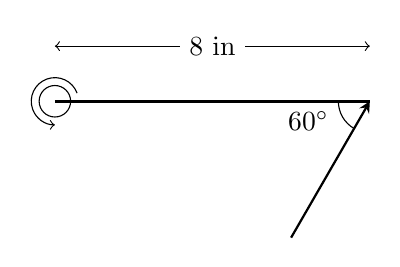
\begin{tikzpicture}[baseline=-1cm]
\draw (0,0) circle (0.2cm);
\draw[->] (20:0.3cm) arc (20:270:0.3cm);
\draw[very thick] (0,0) -- (4,0);
\draw[<->] (0,0.7) -- node[fill=white] {8 in} (4,0.7);
\draw[thick,-stealth] (4,0)+(240:2cm) -- (4,0);
\draw (3.6,0) node[below left] {$60^\circ$} arc (180:240:0.4cm);
\end{tikzpicture}


\begin{solution}[1in] For $P$ at the hinge and $Q$ along the door $8$ inches from $P$, since the torque is
$$\vect{\tau}=\vect{PQ}\times \vect{F} $$
then by the right hand rule, \fbox{the direction of the torque is out of the page towards you}. And the magnitude is:
$$\norm{\vect{\tau}}=\norm{\vect{PQ}}\norm{ \vect{F}}\sin60^{\circ}=\frac{8}{12}(30) \frac{\sqrt{3}}{2}=\boxed{10\sqrt{3}\text{ ft-lbs}} $$
\end{solution}

\end{parts}

\end{problem*}


\end{exam}
\end{document}
